
\documentclass[10pt,twoside,slovak,a4paper]{article}

\usepackage[slovak]{babel}
\usepackage[IL2]{fontenc}
\usepackage[utf8]{inputenc}
\usepackage{graphicx}
\usepackage{url}
\usepackage{hyperref} % odkazy v texte budú aktívne (pri niektorých triedach dokumentov spôsobuje posun textu)

\usepackage{cite}
%\usepackage{times}

\pagestyle{headings}

\title{Využívanie cloudových služieb v 
modernom vyučovacom procese\thanks{Semestrálny projekt v predmete Metódy inžinierskej práce, ak. rok 2020/21, vedenie: Mgr. Martin Sabo, PhD.}} % meno a priezvisko vyučujúceho na cvičeniach

\author{Ján Ágh\\[2pt]
	{\small Slovenská technická univerzita v Bratislave}\\
	{\small Fakulta informatiky a informačných technológií}\\
	{\small \texttt{xagh@stuba.sk}}
	}

\date{\small 20. október 2020} % upravte



\begin{document}

\maketitle

\begin{abstract}

Po digitálnej revolúcii si nové technológie, ako napríklad cloudové služby, postupne
našli svoju cestu aj do každodenného vyučovacieho procesu a v dnešnej dobe sa už považujú
za jeho dôležitú súčasť. Ich inklúzia viedla k vzniku množstva nových situácií, ktorým sa
museli prispôsobiť ako učitelia, tak aj žiaci. Medzi najvýznamnejšie z nich bezpochyby patrí
možnosť zdieľania učebných materiálov, ktorá predstavuje primárnu tému článku, a rovnako
fakt, že žiaci a študenti majú prístup k týmto učebným materiálom aj z pohodlia svojho
domova. Cloudové služby taktiež vytvorili základ pre vznik „virtuálnych tried“, pomocou
ktorých učitelia a študenti dokážu komunikovať aj bez potreby osobného stretnutia sa.
Nemenej dôležité sú aj skutočnosti, že cloudové služby vnášajú chýbajúcu flexibilitu do
vyučovania a podporujú znižovanie nákladov v oblasti informačných systémov.

\end{abstract}



\section{Úvod}




\section{Záver}

\begin{figure}
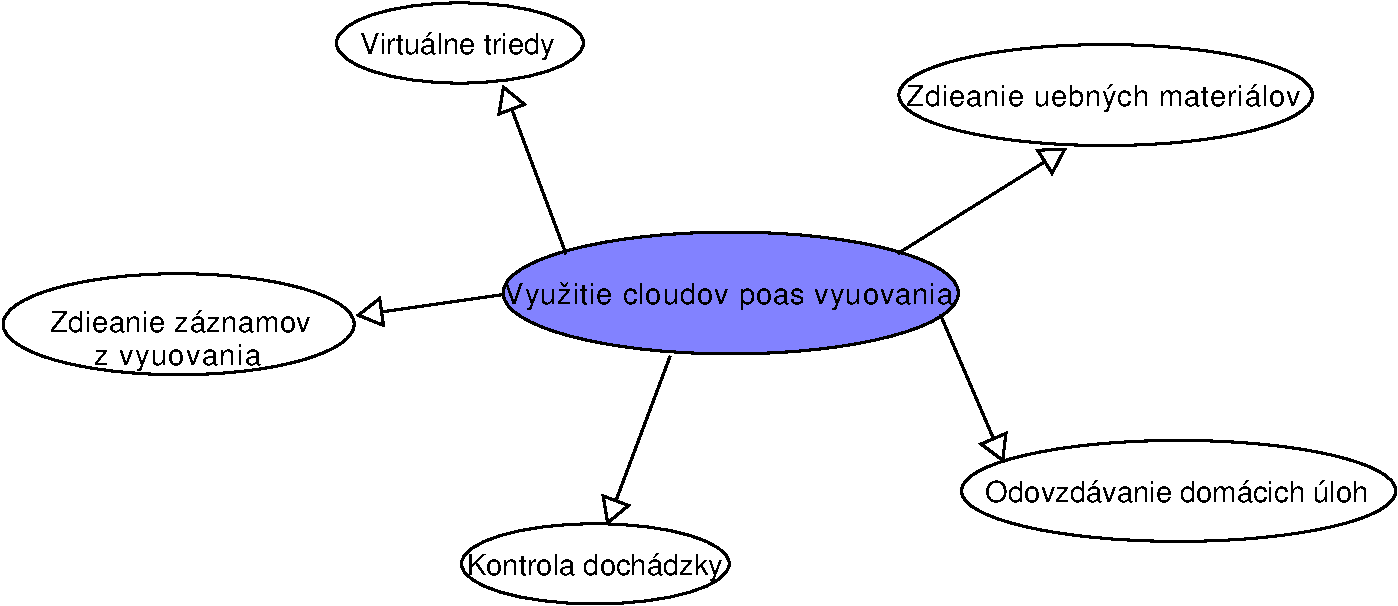
\includegraphics[width=1\textwidth]{Obrázky/opis-crop.pdf}
\caption{Prvý diagram}
\end{figure}


\begin{figure}
\centering
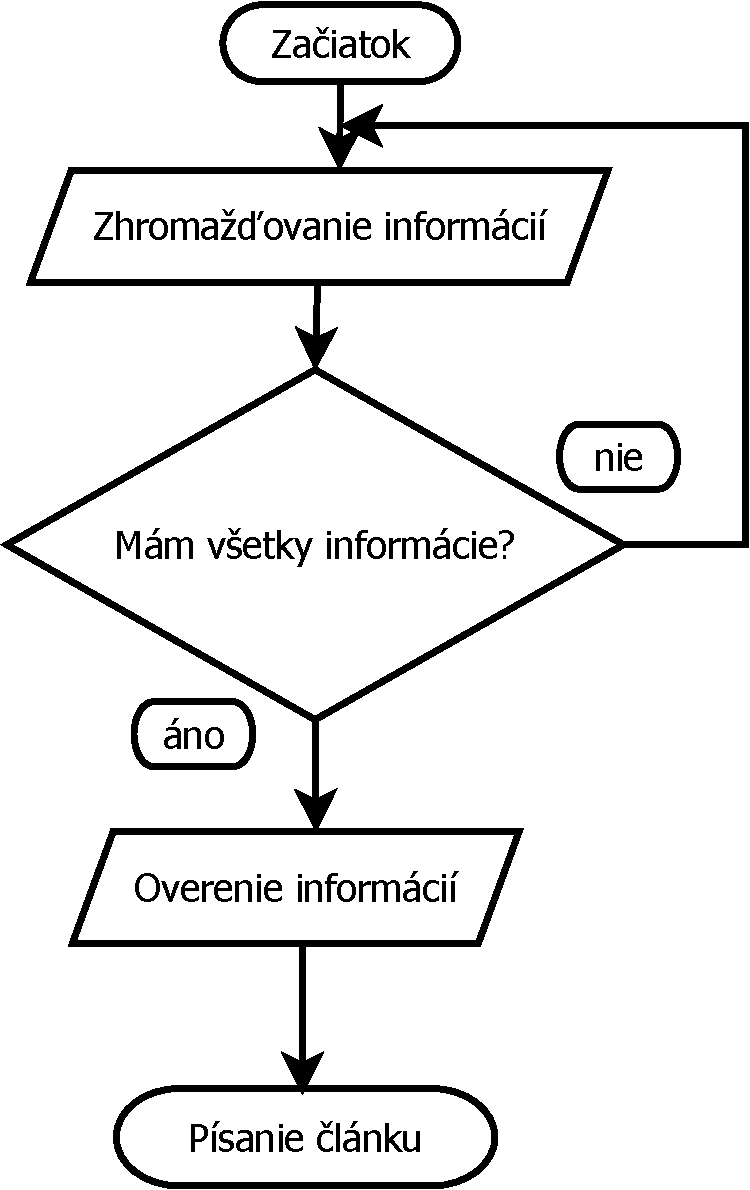
\includegraphics[width=0.5\textwidth]{Obrázky/diagram-crop.pdf}
\caption{Druhý diagram}
\end{figure}


% týmto sa generuje zoznam literatúry z obsahu súboru literatura.bib podľa toho, na čo sa v článku odkazujete
\bibliography{literatura}
\bibliographystyle{plain} % prípadne alpha, abbrv alebo hociktorý iný
\end{document}
